\begin{frame}
    \frametitle{前情回顾}
    \begin{itemize}
        \item 光场量子化~~真空态~~数态~~产生湮灭算符 
        \item 相干态~~压缩态~~辐射场 
        \item 光子计数 ~~ 关联函数~~反聚束
        \item 光场表象
        \item 光与原子相互作用
    \end{itemize}     
\end{frame}

%%%%%%%%%%%%%%%%%%%%%%%%%%%%%%%%%%
\begin{frame} [plain]
    \frametitle{}
    \Background[1] 
    \begin{center}
    {\huge 第18-19讲:光腔中的原子}
    \end{center}  
    \addtocounter{framenumber}{-1}   
\end{frame}


\begin{frame} 
\frametitle{引入}
  \begin{center}
       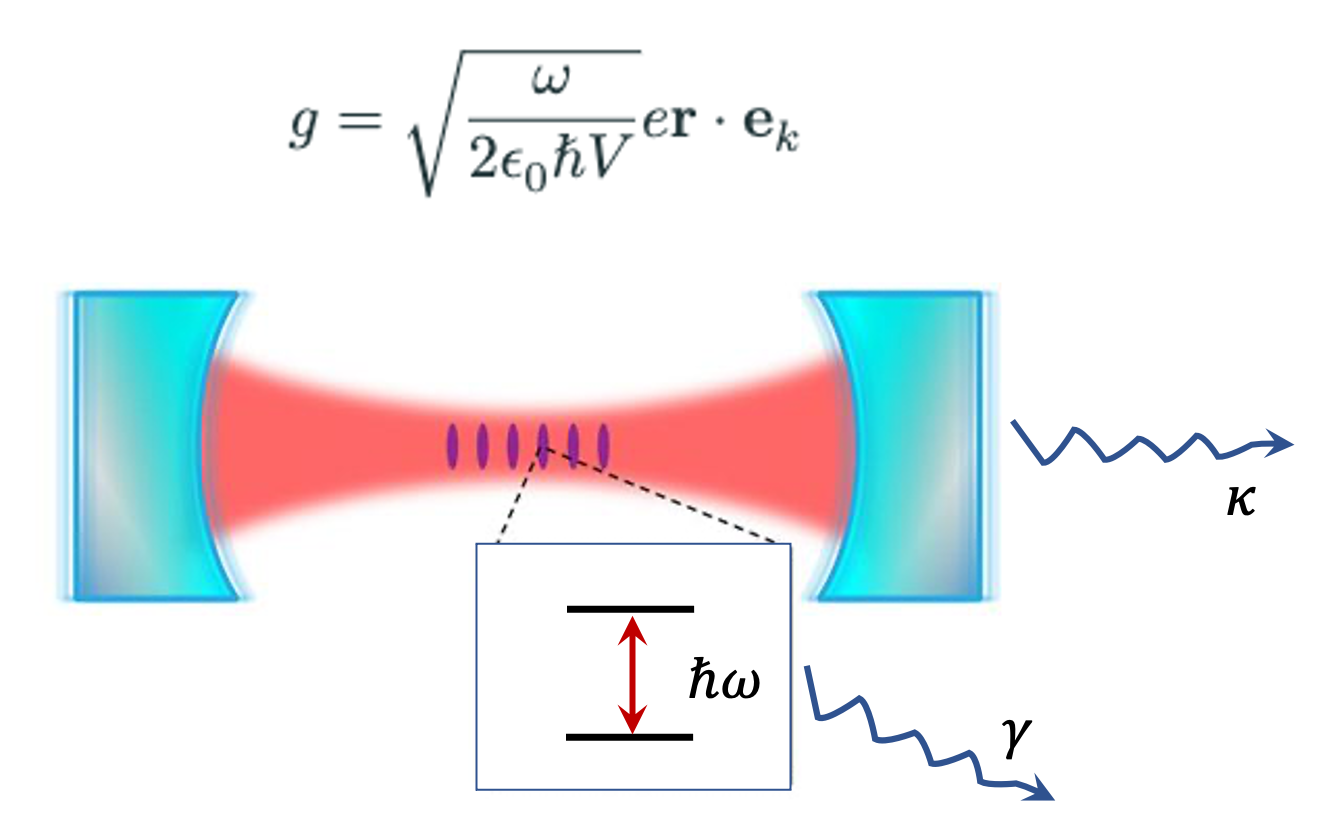
\includegraphics[width=0.6\textwidth]{figs/25.png}
  \end{center}
  想要观察并利用拉比振荡, 必须增强光与原子之间的耦合 $g$. 腔场可最大限度地减少作用体积,增强耦合.
\end{frame}

\section{1. 光学谐振腔}

\begin{frame} 
\frametitle{}   
{\Bullet}光学谐振腔具有选频功能.当不同频率的入射波在腔镜上来回反射时,同频的反射波及入射波之间会相互干涉,腔内稳定传播的都是干涉相长的波.
\begin{columns}[T,onlytextwidth]
    \column{0.59\textwidth}
     考虑fp干涉仪型平面光腔, 透射系数
     \[ T = \frac{1}{1+(4F^2/\pi^2)\sin ^2(\varphi /2)}\]
    式中, 往返相移
    \[ \varphi = \frac{4\pi n L_{cav}}{\lambda}\]
    空腔的精细度
    \[ F = \frac{\pi (R_1 R_2)^{\frac{1}{4}}}{1-\sqrt{R_1 R_2}}\]
    \column{0.4\textwidth}
        \begin{center}
             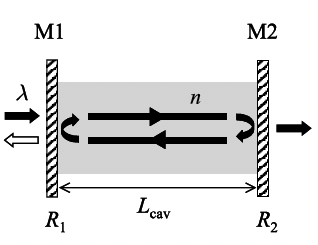
\includegraphics[width=0.9\textwidth]{figs/2022-05-22-23-47-55.png}
        \end{center}
  \end{columns}
\end{frame}

  \begin{frame} 
  \frametitle{}
  \begin{columns}[T,onlytextwidth]
    \column{0.59\textwidth}
       共振透射 ($T=1$) 条件
       \[ \varphi =\frac{4\pi n L_{cav}}{\lambda} = 2 m \pi, \quad m=0, 1, 2, \cdots  \]
       \[L_{cav} = m \frac{\lambda}{2n}\]
       共振模
       \[ \omega_m = m \frac{\pi c }{n L_{cav}}\]
       谱宽
       \[ \Delta \omega = \frac{\pi c }{n F L_{cav}}\]
       品质因数(Q值)
       \[ Q= \frac{\omega}{\Delta \omega }\]
       \column{0.4\textwidth}
       \begin{center}
            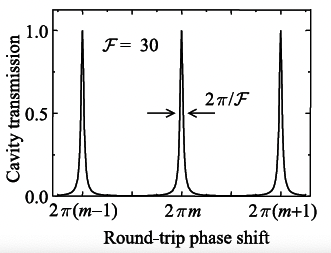
\includegraphics[width=0.9\textwidth]{figs/2022-05-23-00-15-53.png}
       \end{center}
    \end{columns}
  \end{frame}

  \begin{frame} 
  \frametitle{}
    光子寿命
    \[ \tau_{cav} = \frac{n L_{cav}}{c(1-R)}\]
    光子衰减率(损失率)
  \[ \boxed{\kappa \equiv  \frac{1}{\tau_{cav}} = \Delta \omega } \]
       光腔共振模的谱宽由光子衰减率决定 \\ {\vspace*{1.3em}}
       原子光谱的谱宽由原子的自发发射率决定.
       \[ \boxed{A_{21} \equiv  \frac{1}{\tau_{a}} = \Delta \omega } \]
  \end{frame}

  \section{2. 原子与腔的耦合}

\begin{frame} 
\frametitle{}
{\Bullet}若腔内存在原子,腔模与二能级原子共振时, 两者通过交换光子耦合在一起.  \\ {\vspace*{1.3em}}
\begin{columns}[T,onlytextwidth]
    \column{0.59\textwidth}
原子-腔体系最重要的三个参数:
\begin{itemize}
    \item 光子衰减速率 $\kappa = \frac{\omega}{Q}$ 
    \item 非共振衰减速率 $\gamma \equiv \frac{1}{T_2}=  \frac{\gamma_{||}}{2}$
    \item 耦合系数 $g = \sqrt{ \frac{d^2 _{12}\omega}{2  \epsilon_0 \hbar V}}  $
    \end{itemize}
    强耦合条件:
    \[ g \gg \max(\kappa, \gamma) \]
    弱耦合条件:
    \[ g \ll \max(\kappa, \gamma) \]
    \column{0.4\textwidth}
    \begin{center}
     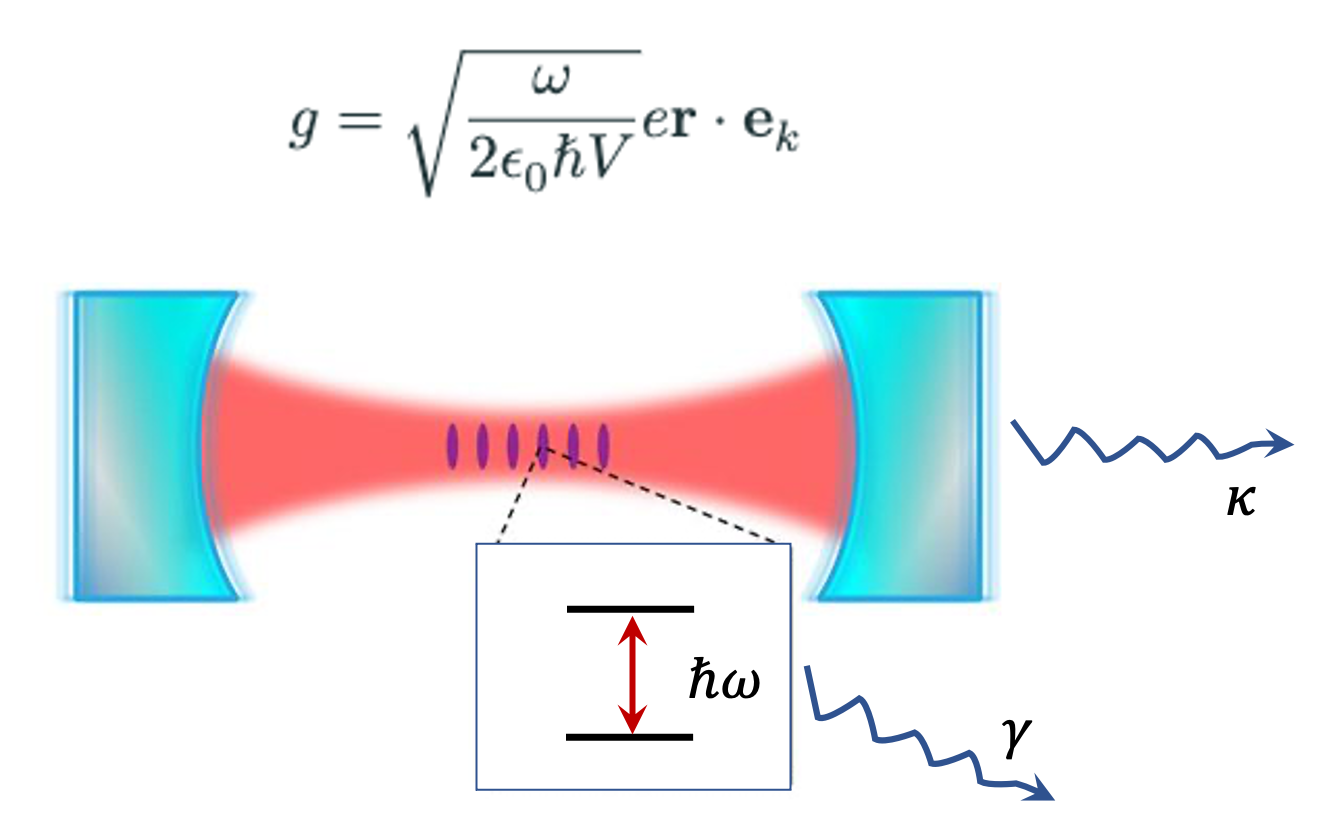
\includegraphics[width=1.0\textwidth]{figs/25.png}
    \end{center}
    \end{columns}
\end{frame}

\begin{frame} 
\frametitle{非共振衰减}
\begin{columns}[T,onlytextwidth]
    \column{0.69\textwidth} 
{\Bullet} 非共振衰减的物理原因: 原子吸收光子后,被激发到激发态. 激发态有一定的寿命, 在这段时间, 可能发生自发发射. 自发发射发出的光的方向是随机的, 不再与腔模共振,导致光子数损失. \\  {\vspace*{1.3em}}
自发发射方向的随机性源于核磁共振(NMR). \\ {\vspace*{1.3em}}
回旋频率(拉莫尔频率)与磁场的关系为
\[ \omega_L = -\gamma B_0\]
$\gamma$称为核回转磁比率
\column{0.3\textwidth}
\begin{center}
 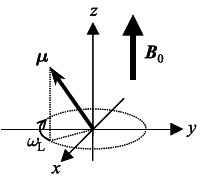
\includegraphics[width=1.0\textwidth]{figs/2022-05-25-11-08-06.png}
\end{center}
\end{columns}
\end{frame}

\begin{frame} 
\frametitle{}
阻尼作用导致这种进动会快速衰减,即最终$M$与$B$平行,进动停止. \\ 腔场的磁分量会策动这种进动,当频率与回旋频率相同当时,发生核磁共振
\[ \mathbf{B}= (B_1)\cos \omega _L t \mathbf{x}\] 
振荡周期为 
\[T = \frac{2\pi}{\gamma B_1 /2} = \frac{4\pi}{\gamma B_1} \] 
对应的频率就是拉比频率
\[ \omega = \frac{\gamma B_1}{4\pi} \]  
  \begin{center}
       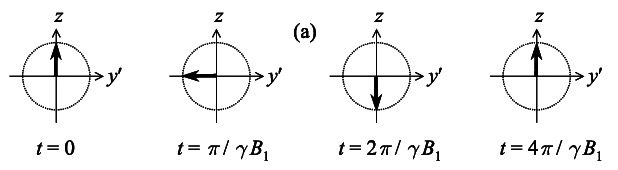
\includegraphics[width=0.8\textwidth]{figs/2022-05-25-11-22-35.png}
  \end{center}
\end{frame}

\begin{frame} 
\frametitle{}
自发发射方向的随机性导致发出的光子与腔模不共振, 损失了光子, 是非共振衰减最重要的因素之一   
  \begin{center}
       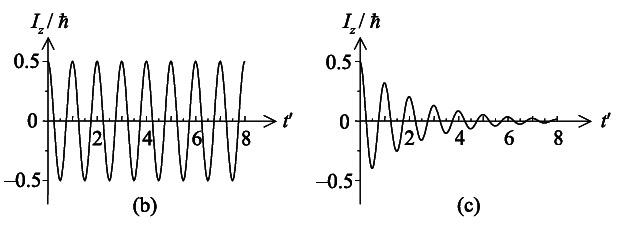
\includegraphics[width=0.8\textwidth]{figs/2022-05-25-11-29-29.png}
  \end{center} 
\end{frame}

\begin{frame} 
\frametitle{}
两种典型散射:
\begin{itemize}
    \item 自旋-晶格弛豫(散射), 周期为 $T_1$
    \item 自旋-自旋弛豫(散射), 周期为 $T_2$
\end{itemize}
自旋-晶格散射过程能量不守恒, 导致$M_z$变小, 也称为纵向松弛. 对应非弹性衰减(可不再发射光子,或发射低频光子). \\ 自旋-自旋散射过程能量守恒, 变化的是 $M_x$,$M_y$, 也称为横向松弛. 对应失相导致的(近)弹性衰减(发射不同相的同频光子).  \\ 
通常,弹性散射(横向弛豫)周期更短,更容易发生.\\ {\vspace*{1.3em}} 
服从布洛赫方程: 
\[ \frac{\mathrm{d} M_i}{\mathrm{d}t} = \gamma (\mathbf{M}\times \mathbf{B}_0)_i - \frac{M_i}{T_2}, \quad i=x,y \]
\[ \frac{\mathrm{d} M_z}{\mathrm{d}t} = \gamma (\mathbf{M}\times \mathbf{B}_0)_z - \frac{M_z - M_0}{T_2} \qquad \]
\end{frame}

\begin{frame} 
\frametitle{}
激发态的寿命由辐射和非辐射衰变两部分构成
\[ \frac{1}{\tau} = \frac{1}{\tau}_R +\frac{1}{\tau}_{NR} \] 
辐射又分弹性辐射和非弹性辐射, 对应$T_1$与$T_2$的关系为:
\[ \frac{1}{T}_2 = \frac{1}{2T}_1+ \frac{1}{T'}_2\]
对于原子-光腔体系, 主要是弹性辐射损失光子. 因此,非共振衰减速率为 \[\gamma \equiv \frac{1}{T_2} =  \frac{\gamma_{||}}{2}\]
立体角内发射的拉比共振光子,因失相造成光子损失.
\[ \gamma_{||} = A_{21}(1- \frac{\Delta \Omega}{4\pi })\] 
当腔长远大于波长时, 立体角很小
\[  \gamma_{||} \approx A_{21}= \frac{1}{\tau}_R\] 
\end{frame}


\begin{frame} 
\frametitle{}
     例: 一个长为60 $\mu m$ 平面光腔内放有一个铯(Cs)原子, 锁定的光场模体系为 $5\times 10 ^{-14} m^3$, 现已知铯的辐射波长为 $852 nm$, 辐射寿命为 32 $ns$, 偶极矩因子$\left|u_{12}\right|= 3\time 10 ^{-29} C \quad m $  \\ 
     (1) 求原子-光腔的耦合系数 $g$ \\
     (2) 非共振衰减速率 $\gamma$  \\ 
     (3) 说明耦合类型 \\ 
    \解 ~(1) 原子-光腔的耦合系数
    \[ \begin{aligned}
        V &= 5\times 10 ^{-14} \,m^3 \\
        \left|u_{12}\right| &= 3\time 10 ^{-29} \,C \quad m \\
        \omega &= \frac{2\pi c}{\lambda} = 2.2\times 10^{15} \,rad\, s^{-1} \\ 
        g &= \sqrt{ \frac{d^2 _{12}\omega}{2  \epsilon_0 \hbar V}} = 1.5 \times 10^8 \,rad\, s^{-1}
    \end{aligned}\] 
    \end{frame}
    
    \begin{frame} 
    \frametitle{}  
    (2) 腔长远大于波长, 
    \[ \begin{aligned} 
        \gamma_{||} & \approx A_{21}= \frac{1}{\tau}_R = \frac{1}{32\times 10^{-9}} s^{-1}=  3.1 \times 10^7  \, s^{-1} \\ 
        \gamma & \equiv \frac{1}{T_2} =  \frac{\gamma_{||}}{2} = 1.6 \times 10^7  \,s^{-1}
    \end{aligned}\] 
    (3) $ g = 1.5 \times 10^8, \gamma= 1.6 \times 10^7$, 有 $g \gg \gamma$, 因此原子与光腔是强耦合的.
\end{frame}

\section{3. 弱耦合与珀塞尔效应}

\begin{frame} 
\frametitle{}
{\Bullet}弱耦合时, 原子从光场吸收能量, 并以自发发射方式放出能量, 对应场模光子数的快速衰减和自发发射的增强. \\  {\vspace*{2.3em}}
{\Bullet}光场可以看成是对原子体系的微扰, 可基于黄金定则进行自发发射计算.
\[ W = \frac{2\pi}{\hbar^2} \left|M_{12}\right|^2 g(\omega) V_0\]
\end{frame}

    \begin{frame} 
    \frametitle{~3.1 光子态密度 }
        
    \begin{columns}
        \begin{column}[t]{0.69\linewidth} 
                考虑一个体系为$V=L^3$ 的自由空间内的电场做行波分解
                \[ \begin{aligned}
                    \mathbf{E}(\mathbf{r},t) &= \sum _\mathbf{k} E_\mathbf{k} e^{i( \mathbf{k}\cdot \mathbf{r} -\omega t )}\\
                        &= \sum _{k_x, k_y, k_z} E_\mathbf{k} e^{i k_x x }e^{i k_y y } e^{i k_z z }  e^{-i \omega t}
                \end{aligned}\] 
            $\mathbf{k}$空间的量子化条件
            \[ \mathbf{k} = (k_x, k_y, k_z) = \frac{2\pi}{L} (n_x, n_y, n_z), \quad n_i =0, \pm 1, \pm 2, \cdots  \]
            相格的体积为: $(\dfrac{2\pi}{L})^3$. 设 $k$的不确定度为 $d k$, 球壳的体积为 $4 \pi k^2 d k$
        \end{column}
        \begin{column}[t]{0.30\linewidth}
              \begin{center}
                   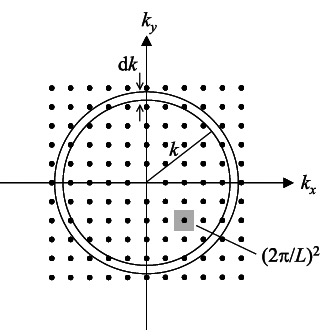
\includegraphics[width=1.0\textwidth]{figs/2022-05-26-11-17-12.png}
              \end{center}
        \end{column}
    \end{columns}
\end{frame}

\begin{frame} 
    \frametitle{}
    球壳内所包含的相格数目(态的数目):
    \[ g(k)^{3D} dk = \frac{4 \pi k^2 d k}{(\dfrac{2\pi}{L})^3} = V \frac{k^2}{2\pi^2} dk\]
    态密度:
    \[ g(k) = \frac{g(k)^{3D}}{V} = \frac{k^2}{2\pi^2}\]
    \[ g(\omega) = \frac{2 \times g(k) dk }{d \omega} = \frac{\omega^2}{\pi^2 c^3}\]
    \[ g(E) = \frac{ g(\omega) d \omega }{d E} = \frac{ g(\omega) }{\hbar}\]
\end{frame}

    \begin{frame} 
    \frametitle{~3.2 自发发射率}
    对于自由空间($V_0$)的原子, 自发发射率 (费米黄金定则): 
    \[ W = \frac{2\pi}{\hbar^2} \left|M_{12}\right|^2 g(\omega) V_0\]
    真空态偶极矩 
    \[ \left|M_{12}\right|^2 =\frac{1}{3} d^2_{12} E^2_{vac} = \frac{d^2_{12} \hbar \omega}{6 \epsilon_0 V_0}\]
    代回, 得自发发射率
    \[ W^{free} \equiv \frac{1}{\tau_R} = A_{21} =  \frac{d^2_{12} \omega ^3 }{3 \pi \epsilon_0 \hbar c^3} \]
    \[ A_{21}=  \frac{ \hbar \omega ^3 }{ \pi ^2 \hbar c^3} B^\omega _{21}\]
    \end{frame}

    \begin{frame} 
    \frametitle{~3.3 珀塞尔效应}
       
           \begin{columns}
               \begin{column}[t]{0.69\linewidth}
                对于如图单模光场, 可归一化  
                \[ \int _0 ^\infty g(\omega) d \omega  = \int _0 ^\infty \frac{\omega^2}{\pi^2 c^3} d \omega =1 \]
                因此, 必满足洛伦兹线型函数 
                \[ g(\omega) = \frac{2}{\pi \Delta \omega_c}  \frac{\Delta \omega_c ^2}{4(\omega -\omega_c)^2 +\Delta \omega_c ^2} \]
               \end{column}
               \begin{column}[t]{0.3\linewidth}
                  \begin{center}
                       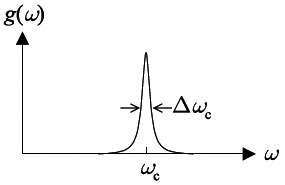
\includegraphics[width=1.0\textwidth]{figs/2022-05-26-12-13-25.png}
                  \end{center}
               \end{column}
           \end{columns}  
    \end{frame}

    \begin{frame} 
    \frametitle{}
    考虑原子与腔场的共振耦合($\omega = \omega_c$)
    \[ g(\omega)  = \frac{2}{\pi \Delta \omega_c} = \frac{2}{\pi \Delta \omega} \frac{\omega_c}{\Delta \omega_c} = \frac{2Q}{\pi \omega} \]
    令 \[\xi = \frac{\left| e \mathbf{r} \cdot \mathbf{E} \right|}{\left|e \mathbf{r}\right| \left| \mathbf{E}\right|} \]
    光子态的偶极矩 
    \[ \left|M_{12}\right|^2 = \xi^2 d^2_{12} E^2_{vac} = \frac{d^2_{12} \hbar \omega}{2 \epsilon_0 V_0}\]
    代回费米黄金定则, 腔场中原子的自发发射率
    \[ W^{cav} =  \frac{ 2 Q d^2_{12}}{ \hbar \epsilon_0 } \, \xi^2  \,  \frac{\Delta \omega_c ^2}{4(\omega -\omega_c)^2 +\Delta \omega_c ^2} \]
    \end{frame}

    \begin{frame} 
    \frametitle{}
        定义珀塞尔因子(Purcell~factor)
        \[ F_P \equiv  \frac{W^{cav}}{W^{free}} \equiv \frac{W^{free} _R }{\tau^{cav} _R} \]
        得:
        \[ F_P = \frac{ 3 Q (\lambda /n) ^3}{ 4 \pi^2 V_0 } \, \xi^2  \,  \frac{\Delta \omega_c ^2}{4(\omega -\omega_c)^2 +\Delta \omega_c ^2}  \]
        完全共振时
        \[ F_P = \frac{ 3 Q (\lambda /n) ^3}{ 4 \pi^2 V_0 }  \]
        \begin{itemize}
            \item 当 $F_P > 1$, 偶合增强了原子的自发发射
            \item 当 $F_P < 1$, 偶合消弱了原子的自发发射
        \end{itemize}  
        {\Bullet}增强条件: (1)高Q值, (2)低模态体积$V_0$, (3) 近共振 $\omega \approx \omega_c$, (4) 偶极矩与场模尽量平行 $\xi ^2$
    \end{frame}

    \begin{frame} 
        \frametitle{}
        \begin{columns}
            \begin{column}[t]{0.69\linewidth}
            考虑到 $W= W^{cav} + W^{free} $ (如图)  \\  {\vspace*{1.3em}}
            定义自发发射耦合因子
            \[ \beta \equiv  \frac{W^{cav}}{W^{cav} + W^{free}} = \frac{F_P}{1+F_P} \]
            当 $F_P$  很大时, $\beta \to 1$, 偶合增强自发发射率. \\ {\vspace*{1.3em}}

            实验上通常通过在构造极小的模态体积$V_0 \sim \lambda /n $, 以实现珀塞尔效应 (如右图).
            \end{column}
            \begin{column}[t]{0.3\linewidth}
                  \begin{center}
                       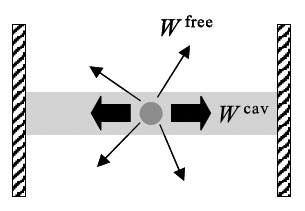
\includegraphics[width=1.0\textwidth]{figs/2022-05-26-14-21-39.png}
                       ~\\
                       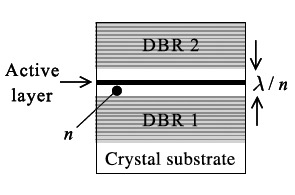
\includegraphics[width=1.0\textwidth]{figs/2022-05-26-14-49-23.png}
                  \end{center}
            \end{column}
        \end{columns}
    \end{frame}
\section{4. 强耦合与拉比劈裂}

\begin{frame} 
\frametitle{~4.1 哈密顿的矩阵表示}
    强耦合体系, 光与原子的相互作用能不能看成微扰, 因此不能利用黄金定则进行计算.  \\ 
    体系的哈密顿为: 
    \[\begin{aligned}
        H &= \hbar \omega S_z + \hbar \omega_0 (a^{\dagger}  a +\frac{1}{2}) + \hbar g ( a S^- + S^+ a ^{\dagger}) 
    \end{aligned} \] 
    能量简并的两个非缀饰基矢态:
    \[ \rs{\psi_1} = \rs{n, 1}, \qquad \rs{\psi_2} =\rs{n-1, 2},  \] 
\end{frame}

\begin{frame} 
\frametitle{}
哈密顿在非缀态表象中矩阵表示
    \[ \begin{aligned}
        H_{11} & =  \ls{\psi_1} H \rs{\psi_1} =  \ls{1,n} H \rs{n, 1} = \hbar n \omega_0 +\frac{1}{2} \hbar \Delta \\
        H_{22} & =  \ls{\psi_2} H \rs{\psi_2} =  \ls{2,n-1} H \rs{n-1, 2} = \hbar n \omega_0 -\frac{1}{2} \hbar \Delta \\
        H_{12} & =  \ls{\psi_1} H \rs{\psi_2} =  \ls{1,n} H \rs{n-1, 2} = \frac{1}{2} \hbar g \sqrt{n} \\
        H_{21} & =  \ls{\psi_2} H \rs{\psi_1} =  \ls{2,n-1} H \rs{n, 1} = \frac{1}{2} \hbar g \sqrt{n} \\ 
    \end{aligned}\]  
* 式中,  $\Delta = \omega -\omega_0 $ 是失谐频率, $\Omega = g \sqrt{n}$ 是拉比频率. \\ 
* 耦合效应体现在非对称元上. \\
* 计算过程略
\end{frame}

\begin{frame} 
\frametitle{}
    对于共振体系($\Delta = \omega -\omega_0 =0 $)\\ 
    哈密顿矩阵为:
    \[ H = \begin{bmatrix}
        \hbar n \omega  & \frac{1}{2} \hbar g \sqrt{n} \\
        \frac{1}{2} \hbar g \sqrt{n} & \hbar n \omega
     \end{bmatrix}\]
    解久期方程, 得能量本征值:
    \[ E^{\pm} = \hbar n \omega \pm \frac{1}{2} \hbar g \sqrt{n} \]
\end{frame}

\begin{frame} 
    \frametitle{~4.2 缀饰态}
    能量本征态(缀饰态)用非缀饰态的叠加态展开 
    \[ \rs{\Psi_n} = a \rs{n, 1} + b\rs{n-1, 2} = \begin{bmatrix}
        a\\
        b 
     \end{bmatrix}\]
     解方程 
     \[ \begin{bmatrix}
        \hbar n \omega - E^{\pm}  & \frac{1}{2} \hbar g \sqrt{n} \\
        \frac{1}{2} \hbar g \sqrt{n} & \hbar n \omega -E^{\pm} 

     \end{bmatrix}        
     \begin{bmatrix}
            a \\
            b
         \end{bmatrix}
         =0\] 
得两本征态 
 \[\rs{\Psi_{n\pm}} = \frac{1}{\sqrt{2}} \left(\rs{n, 1} \pm \rs{n-1, 2}\right)\]
\end{frame}

\begin{frame} 
    \frametitle{~4.3 拉比劈裂}
   \begin{center}
        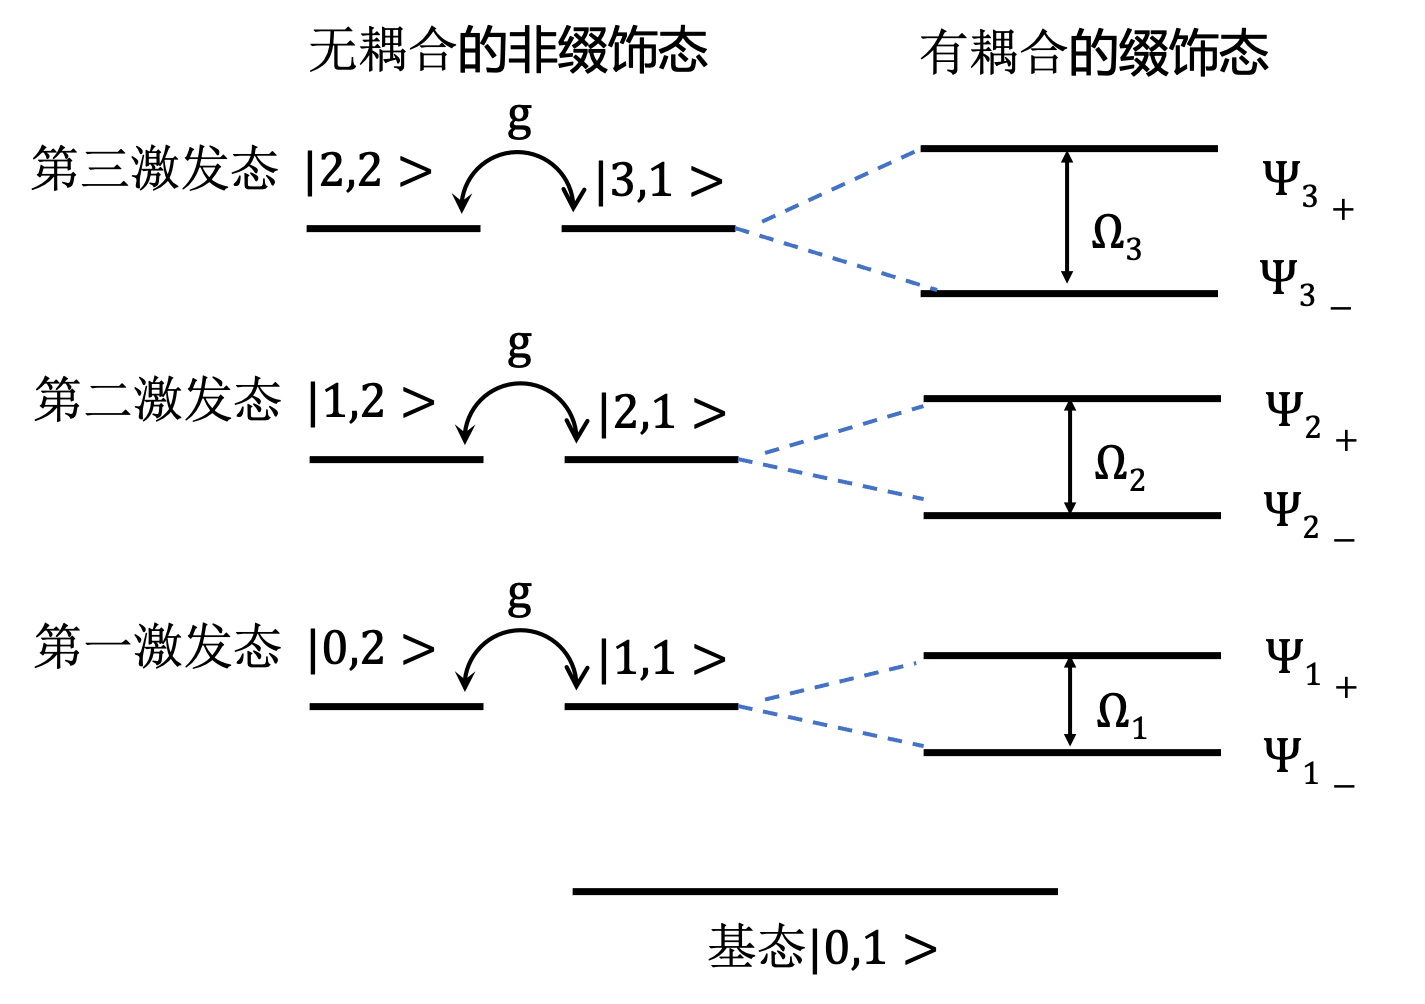
\includegraphics[width=0.78\textwidth]{figs/27.png}
   \end{center}
   *拉比劈裂也称塞曼效应
\end{frame}

\begin{frame} 
    \frametitle{}
        对于非共振(失谐)体系($\Delta = \omega -\omega_0 \not =0 $)\\ 
     能量本征值
        \[ E^{\pm} = \hbar n \omega \pm  \hbar \sqrt{ \Delta ^2 + \frac{1}{4} n g ^2 } \]
    能量本征态(缀饰态)
    \[\begin{aligned}
        \rs{\Psi_{n+}} & =  \sin \theta \rs{n, 1} + \cos \theta  \rs{n-1, 2} \\ 
        \rs{\Psi_{n-}} & =  \cos  \theta \rs{n, 1} - \sin \theta  \rs{n-1, 2} \\ 
    \end{aligned} \]
    式中, \[ \cos \theta = \frac{ \Omega - \Delta}{(\Omega - \Delta)^2 + 4g^2 n } \]
    \end{frame}

    \begin{frame} 
    \frametitle{}
    缀饰态能量与失谐频率的关系:
      \begin{center}
           \includegraphics[width=0.6\textwidth]{figs/28.png}
      \end{center} 
      两缀饰态的能量不能有交叉
    \end{frame}

    \begin{frame} 
    \frametitle{实验验证}
     光子晶体:
       \begin{center}
            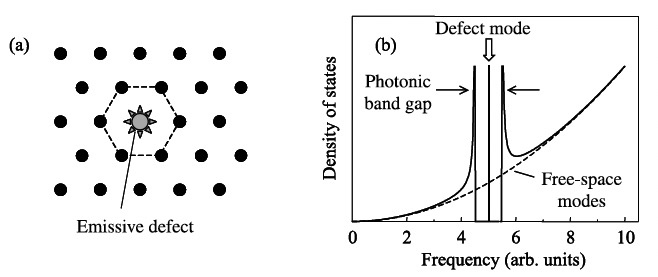
\includegraphics[width=0.9\textwidth]{figs/2022-05-27-21-03-17.png}
       \end{center}       
    \end{frame}

    \begin{frame} 
    \frametitle{}
           \begin{center}
                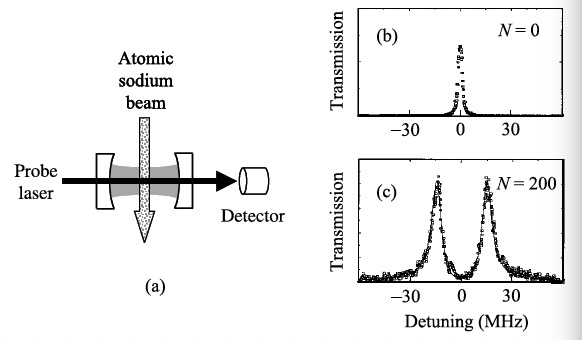
\includegraphics[width=0.8\textwidth]{figs/2022-05-27-21-07-24.png}
           \end{center}
        (a) 装置图   (b) 空腔模  (c) 平均~200~个钠原子
    \end{frame}
